% !TEX root = main.tex
\chapter{Real time decoder}
\label{cha:decoder}

This chapter describes the implementation
of the new {\it OnlLatticeFasterDecoder}\/ and 
the modification of an online speech parametrisation and feature transformations.

We limited our task, so it fits our requirements for real time decoding
in our \ac{SDS} Alex.
We need a real time decoder with sufficient accuracy,
which does not apply any speaker adaptive transformations.
We strongly prefer n-best list or lattice output formats over one-best hypothesis.
In addition, we require latency under 0.2 seconds after the end of user speech.

We also wanted to reuse existing code as much as possible,
so the decoder will benefit from constant development on Kaldi toolkit.
As a bonus of the minimal changes we can compare our {\it OnlLatticeFasterDecoder}\/ 
with {\it LatticeFasterDecoder}\/ which is used through binary executable {\it gmm-latgen-faster}.
Correctly setup, the decoders produce exactly the same results.


\section{Online pre-processing} 
\label{sec:onl_preprocess}
The pre-processing consist of audio signal buffering, \ac{MFCC} feature extraction and
applying feature transformation. 
The pre-processing and the decoder are bridged by the {\it decodable} 
interface as illustrated in Figure~\ref{fig:online_pipeline}.
We briefly describe each step:
\begin{itemize}
    \item Audio buffering
    \item Computation of \ac{MFCC} features
    \item Applying feature transformation. 
        \begin{itemize}
            \item $\Delta + \Delta\Delta$ \todo{How many frames requires}
            \item The $LDA+MLLT$ is computed using context,
                which by default is set to four previous and four future frames.
        \end{itemize}
        Note, that the $LDA+MLLT$ and the $\Delta+\Delta\Delta$ transformations are complementary.
    \item The {\it Decodable}\/ interface in our case the its {\it OnlDecodableDiagGmmScaled}\/ implementation
        queries the \ac{AM} for the probability for acoustic features $a$ and given state.
        Note that the acoustic features $a$ are the output of the previous steps.
    \item The decoder itself performs the search in state level space 
        having the probabilities from the {\it Decodable}\/ interface. 
        States represents triphones where for some thriphones the parameters are shared.
\end{itemize}

\begin{figure}[!htp]
    \begin{center}
        \psscalebox{1.0 1.0} % Change this value to rescale the drawing.
{
\begin{pspicture}(0,-2.1866903)(14.64,2.1866903)
\rput[bl](6.316553,0.59188676){TODO}
\end{pspicture}
}

        \caption{Components for online decoding}
    \label{fig:online_pipeline} 
    \end{center}
\end{figure}

Each step in~Figure~\ref{fig:online_pipeline} is implemented as a class.
In Figure~\ref{fig:classes} you may see, that additional helper class is also used.
During decoding each class is instantiated only once at the beginning.
The pre-processing classes are aggregated together. 
The {\it OnlBuffSource}\/ is setup as member of {\it OnlFeInput<Mfcc>}\/.
The {\it OnlFeInpute<Mfcc>}\/ is setup as member of either {\it OnlLdaInput}\/ or {\it OnlDeltaInput}\/.
One of the transformations is setup as member to {\it OnlFeatureMatrix}\/ instance.

The {\it OnlLatticeFasterDecoder}\/ performs forward decoding frame by frame using the Viterbi beam search.
The forward decoding is performed on request by calling the method {\it decode(int max\_frames)}.
It returns the number of frames which were actually decoded, which is always smaller than {\it max\_frames}.
In order to evaluate the probability of acoustic features for the new frame
the decoder query the {\it Decodable}\/ interface.

\begin{figure}[!htp]
    \begin{center}
        % Graphic for TeX using PGF
% Title: /home/ondra/Diagram1.dia
% Creator: Dia v0.97.2
% CreationDate: Thu Aug  1 08:02:11 2013
% For: ondra
% \usepackage{tikz}
% The following commands are not supported in PSTricks at present
% We define them conditionally, so when they are implemented,
% this pgf file will use them.
\ifx\du\undefined
  \newlength{\du}
\fi
\setlength{\du}{15\unitlength}
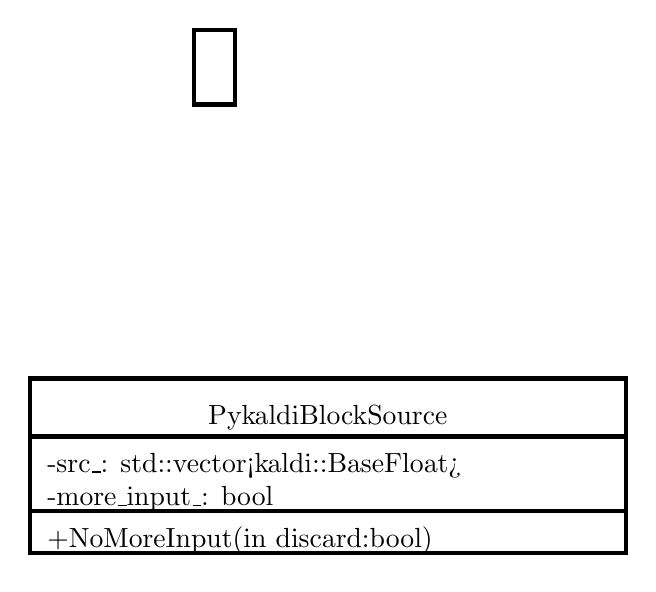
\begin{tikzpicture}
\pgftransformxscale{1.000000}
\pgftransformyscale{-1.000000}
\definecolor{dialinecolor}{rgb}{0.000000, 0.000000, 0.000000}
\pgfsetstrokecolor{dialinecolor}
\definecolor{dialinecolor}{rgb}{1.000000, 1.000000, 1.000000}
\pgfsetfillcolor{dialinecolor}
\pgfsetlinewidth{0.100000\du}
\pgfsetdash{}{0pt}
\definecolor{dialinecolor}{rgb}{1.000000, 1.000000, 1.000000}
\pgfsetfillcolor{dialinecolor}
\fill (13.250000\du,6.900000\du)--(13.250000\du,8.700000\du)--(14.250000\du,8.700000\du)--(14.250000\du,6.900000\du)--cycle;
\definecolor{dialinecolor}{rgb}{0.000000, 0.000000, 0.000000}
\pgfsetstrokecolor{dialinecolor}
\draw (13.250000\du,6.900000\du)--(13.250000\du,8.700000\du)--(14.250000\du,8.700000\du)--(14.250000\du,6.900000\du)--cycle;
% setfont left to latex
\definecolor{dialinecolor}{rgb}{0.000000, 0.000000, 0.000000}
\pgfsetstrokecolor{dialinecolor}
\node at (13.750000\du,7.995000\du){};
% setfont left to latex
\pgfsetlinewidth{0.050000\du}
\definecolor{dialinecolor}{rgb}{0.000000, 0.000000, 0.000000}
\pgfsetstrokecolor{dialinecolor}
\draw (13.750000\du,8.147500\du)--(13.750000\du,8.147500\du);
\pgfsetlinewidth{0.100000\du}
\pgfsetdash{}{0pt}
\definecolor{dialinecolor}{rgb}{1.000000, 1.000000, 1.000000}
\pgfsetfillcolor{dialinecolor}
\fill (9.300000\du,15.300000\du)--(9.300000\du,16.700000\du)--(23.660000\du,16.700000\du)--(23.660000\du,15.300000\du)--cycle;
\definecolor{dialinecolor}{rgb}{0.000000, 0.000000, 0.000000}
\pgfsetstrokecolor{dialinecolor}
\draw (9.300000\du,15.300000\du)--(9.300000\du,16.700000\du)--(23.660000\du,16.700000\du)--(23.660000\du,15.300000\du)--cycle;
% setfont left to latex
\definecolor{dialinecolor}{rgb}{0.000000, 0.000000, 0.000000}
\pgfsetstrokecolor{dialinecolor}
\node at (16.480000\du,16.250000\du){PykaldiBlockSource};
\definecolor{dialinecolor}{rgb}{1.000000, 1.000000, 1.000000}
\pgfsetfillcolor{dialinecolor}
\fill (9.300000\du,16.700000\du)--(9.300000\du,18.500000\du)--(23.660000\du,18.500000\du)--(23.660000\du,16.700000\du)--cycle;
\definecolor{dialinecolor}{rgb}{0.000000, 0.000000, 0.000000}
\pgfsetstrokecolor{dialinecolor}
\draw (9.300000\du,16.700000\du)--(9.300000\du,18.500000\du)--(23.660000\du,18.500000\du)--(23.660000\du,16.700000\du)--cycle;
% setfont left to latex
\definecolor{dialinecolor}{rgb}{0.000000, 0.000000, 0.000000}
\pgfsetstrokecolor{dialinecolor}
\node[anchor=west] at (9.450000\du,17.400000\du){-src\_: std::vector<kaldi::BaseFloat>};
% setfont left to latex
\definecolor{dialinecolor}{rgb}{0.000000, 0.000000, 0.000000}
\pgfsetstrokecolor{dialinecolor}
\node[anchor=west] at (9.450000\du,18.200000\du){-more\_input\_: bool};
\definecolor{dialinecolor}{rgb}{1.000000, 1.000000, 1.000000}
\pgfsetfillcolor{dialinecolor}
\fill (9.300000\du,18.500000\du)--(9.300000\du,19.500000\du)--(23.660000\du,19.500000\du)--(23.660000\du,18.500000\du)--cycle;
\definecolor{dialinecolor}{rgb}{0.000000, 0.000000, 0.000000}
\pgfsetstrokecolor{dialinecolor}
\draw (9.300000\du,18.500000\du)--(9.300000\du,19.500000\du)--(23.660000\du,19.500000\du)--(23.660000\du,18.500000\du)--cycle;
% setfont left to latex
\definecolor{dialinecolor}{rgb}{0.000000, 0.000000, 0.000000}
\pgfsetstrokecolor{dialinecolor}
\node[anchor=west] at (9.450000\du,19.200000\du){+NoMoreInput(in discard:bool)};
\end{tikzpicture}

    \caption{Aggregation of classes for serial input processing}
    \label{fig:classes} 
    \end{center}
\end{figure}

In case of {\it OnlDecodableDiagGmmScaled}, the online implementation, can trigger chain reaction.
If {\it OnlFeatureMatrix}\/ does not contain the acoustic features for the new frame, it asks
the previous component to compute the features, namely {\it OnlDeltaInput}\/ or {\it OnlLdaInput}\/.
If the previous component can not provide the features, it return default empty value indicating,
that no features are not available at the moment. It triggers the message that no data is available
and the decoder's method {\it decode(..)}, returns zero, meaning that no frames were decoded.

\subsubsection{History and work implemented}
\label{ssub:history}
We did not implemented the classes {\it OnlDeltaInput, OnlLdaInput, OnlFeInput}\/ and {\it OnlFeatureMatrix}\/
from scratch. We started the work with Mathias Pawlik implementation and we implemented few buffering details
in the classes, but mainly we removed the built in timeouts and changed the interface.
Note that we also added the {\it OnlBuffSource}\/ class, which just allows buffer the raw \ac{PCM} audio.

Let us argue why using timeouts is not convenient in the speech recognizing code
and should be let to the code which uses the speech recoginition code.
Our \ac{API} immediatly reports there are no frames available.
On the other hand in the code with timetouts, you have to wait the {\it timeout}\/ time
in order to figure out that there are no frames available.
In addition, if you have timetouts in multiple preprocessing classes the timeouts time may chain.
Finally, the timeouts require reinitialization of the preporcessing classes with frame context,
because the user did not respond during the {\it timeout}\/. 
Obviously, the delay could be caused by other reasons. For example if the application, 
which uses the speech recognition engine sends the audio over network, the network can be
the cause of exceeding the {\it timeout}\/.

\section{Online decoder interface} 
\label{sec:improve}
We started developing the real-time speech recognizer by preparing the preprocessing
pipeline as describe in~Section~\ref{sec:onl_preprocess}, after that we focused 
on implementation the real time decoder. In the first step we changed 
the batch {\it LatticeFasterDecoder}\/ only by reorganizing its methods into new interface.
It turned out that the decoder with the new interface is 
fast enough and sufficiently accurate for \ac{SDS}. 
The evaluation in \ac{SDS} Alex is described in~Section~\ref{sec:evalution}.

Let us describe the details how we reorganized the {\it LatticeFasterDecoder}\/ 
into {\it OnlLatticeFasterDecoder}.

\begin{figure}[!htp]
    \begin{center}
        \begin{verbatim}
class LatticeFasterDecoder {
 public:
  // Returns true if any kind of traceback is available (not necessarily from
  // a final state).
  bool Decode(DecodableInterface *decodable);

  /// says whether a final-state was active on the last frame.  If it was not, the
  /// lattice (or traceback) will end with states that are not final-states.
  bool ReachedFinal() const { return final_active_; }

  // This function is now deprecated, since now we do determinization from
  // outside the LatticeTrackingDecoder class.
  // Outputs an FST corresponding to the lattice-determinized
  // lattice (one path per word sequence).
  bool GetLattice(fst::MutableFst<CompactLatticeArc> *ofst) const;

 protected:
  // There are various cleanup tasks... the the toks_ structure contains
  // singly linked lists of Token pointers, where Elem is the list type.
  // It also indexes them in a hash, indexed by state (this hash is only
  // maintained for the most recent frame).  toks_.Clear()
  // deletes them from the hash and returns the list of Elems.  The
  // function DeleteElems calls toks_.Delete(elem) for each elem in
  // the list, which returns ownership of the Elem to the toks_ structure
  // for reuse, but does not delete the Token pointer.  The Token pointers
  // are reference-counted and are ultimately deleted in PruneTokensForFrame,
  // but are also linked together on each frame by their own linked-list,
  // using the "next" pointer.  We delete them manually.
  void DeleteElems(Elem *list);

  void ClearActiveTokens();

  /// Processes nonemitting (epsilon) arcs for one frame.
  /// Ccalled after ProcessEmitting on each frame.
  /// TODO: could possibly add adaptive_beam back as an argument here (was
  /// returned from ProcessEmitting, in faster-decoder.h).
  void ProcessNonemitting(int32 frame);
            
  /// Processes emitting arcs for one frame.  Propagates from prev_toks_ to cur_toks_.
  void ProcessEmitting(DecodableInterface *decodable, int32 frame);

  // Go backwards through still-alive tokens, pruning them.  note: cur_frame is
  // where hash toks_ are (so we do not want to mess with it because these tokens
  // don't yet have forward pointers), but we do all previous frames, unless we
  // know that we can safely ignore them because the frame after them was unchanged.
  // delta controls when it considers a cost to have changed enough to continue
  // going backward and propagating the change.
  // for a larger delta, we will recurse less far back
  void PruneActiveTokens(int32 cur_frame, BaseFloat delta);

  /// Version of PruneActiveTokens that we call on the final frame.
  /// Takes into account the final-prob of tokens.
  void PruneActiveTokensFinal(int32 cur_frame);
        \end{verbatim}
        \caption{Simplified original interface of {\it LatticeFasterDecoder}\/ with comments.}
    \label{fig:lattice_decoder} 
    \end{center}
\end{figure}

We implemented the new interface by inheriting the {\it OnlLatticeFasterDecoder}\/ from {\it LatticeFasterDecoder}\/ 
and splitting the original {\it bool Decode(DecodableInterface *d)}\/ function 
into three simpler public functions.
\begin{itemize}
    \item {\it size\_t Decode(DecodableInterface *d, size\_t max\_frames)}\/ 
        Decodes using the function calls:
        \begin{itemize}
            \item {\it ProcessEmitting(decodbale, frame\_)}\/ process non $\epsilon$ arcs.
            \item {\it ProcessNonemitting(frame\_)}\/ process $\epsilon$ arcs.
            \item {\it PruneActiveTokens(frame\_, lattice\_beam * 0.1)}\/ Prune still-alive tokens. 
        \end{itemize}

    \item {\it void PruneFinal()}\/ calls {\it PruneActiveTokensFinal(frame\_- 1)}\/, which starts
        with probability of the final tokens and go backwards pruning the tokens.
    \item {\it void Reset()}\/ empties the data structures and turns the decoder into
        initial state.
\end{itemize}

\subsection*{Online interface use case}
The {\it OnlLatticeFasterDecoder}\/ performs forward decoding using 
the~{\it Decode(DecodableInterface *, size\_t max\_frames)}\/.
The function {\it PruneFinal}\/ performs the final pruning and prepares the active tokens from beam,
to be transformed to state level lattice using the backward decoding.
We use the {\it GetLattice(fst::MutableFst<CompactLatticeArc> *ofst)}\/ function,
because the {\it CompactLattice}\/ it efficiently performs 
state level lattice determinisation.\cite{povey2012generating}.

The {\it Reset()} function may be useful, if there is too many unprocessed frames,
so we want to discard all the buffered audio. It is typically the case,
when we did not have enough CPU resources and new user input appears and we want to process
the latest audio input. If a \acl{SDS} has to choose which audio chunk to process, typically the last audio
chunk is the most important for a conversation and the previous chunks are simply discarded.

\code{Usage of the~{\it OnlLatticeFasterDecoder}\/ in its wrapper}{C}{snippets/onl_lat_dec_usage.cc}

\section{Post-processing the state lattice}
\label{sec:postprocess}
% \todo{The trick with discarding alignments}
% \todo{How I converted the state lattice to word posterior lattice}
% \todo{decoding lattices and normal outputs -- describe again the problems}
The {\it CompactLattice}\/ determinised at state level still may contain
multiple paths for each word sequence encoded in the lattice.
In fact, typically there is number of state level alternatives for each word sequence.
We need to realize that the phones are not represented individually at the state level
and we does not concatenate the phone labels on path in order to obtain words and sentences.
The words label is located on the first arc of the word \ac{HMM}. 
The rest of the arcs in the graph are $\epsilon$ transition.

\ml{alignment}
Note that \ac{HMM} states are time synchronous, so traversing one arc represent a fixed time slot.
The time slot corresponds to frame shift as introduced in~Subsection~\ref{sub:param}.
The mapping between each word and the number of arcs from beginning of the utterance is called
alignment.

The {\it CompactLattice}\/ distinguishes each path not only according word labels on the path,
but also according the alignments.
In order to obtain only the word lattice we discard the alignments.
In next steps we convert the {\it CompactLattice}\/ to standard OpenFST object.\footnote{Kaldi implements a special semiring for {\it CompactLattice}\cite{povey2012generating}.}  

The following steps convert the weights on the lattice from representing likelihood
to posterior probabilities. The posterior probabilities are of course approximation of
true posterior probabilities for individual paths in lattice. 

The first approximation has a very small impact. The first approximation is 
that we are using only the lattice constructed from the active states in beam search
and not the complete search space. 
The discarded hypotheses have very low posterior probabilities, so it does a little harm.

More serious problem is violating the assumption that the \ac{AM} and \ac{LM} models are 
computing the true likelihood. 
In generative models we are training and improving the models so the likelihood match
the reality as much as possible.
On contrary, the discriminative \ac{AM} models deliberately favor the most probable hypothesis,
so they are not computing the true likelihood.
The discriminative behaviour can be compensated, but we do not solve the problem
in the decoder, because the decoder has no information, which \ac{AM} was used.

\code{Converting {\it CompactLattice}\/ to posterior word lattice}{C}{snippets/compact2wordpost.cc}

The computing of the posterior probabilities is done through
standard forward-backward algorithm\cite{todo}.
We reused Kaldi function for computing helper $\alpha$ and $\beta$ data structures,
but we implemented the {\it MovePostToArcs}\/ function for updating the lattice weights 
from likelihood to posterior probabilities based on $\alpha$ and $\beta$.

\section{Objected oriented interface to speech recognition}
\label{sec:ooi}
The components of the Kaldi library such as decoder, or \ac{MLLT} transformation are designed using 
the \ac{OOP} design patterns.
On the other hand, the functionality of the Kaldi library is accessed by Kaldi executables, 
which are typically organized into single function.
The Kaldi executables are thin wrappers around the classes and 
are further combined together using system tools e.g.\ system pipes
and storing intermediate results to files. 
Such setup is convenient for speech recognition experiments, because the intermediate results are  
effectively reused by different experiments.

Out task is to implement real-time speech recogniser into \acl{SDS}.
We also experimented and searched for the best setup as described in~Section~\ref{sec:evaluation},
but from the \ac{SDS} point of view we want simple component which accepts audio and produce \ac{ASR} hypothesis.
We profit from the reference {\it LatticeFasterDecoder}, where the Kaldi preprocessing executables
can be scripted in a such manner, so that the results of {\it LatticeFasterDecoder}\/ 
and wrapped {\it OnlLatticeFasterDecoder}\/ are identical.
We used the Kaldi executables to find the best experiment and once fixed,
we created object wrapper around the whole recognition pipeline.

Let us described the Kaldi executable in our best experiment,
then we will describe the wrapper class for the speech recognition.
We chose \ac{MFCC} speech parametrisation, \ac{LDA} and \ac{MLLT} feature transformations with 
acoustic model trained by \ac{bMMI} as our best setup.
In our experiments, we used Kaldi binaries, which are listed below, 
for computing the one best \ac{ASR} hypothesis:
% \todo{How I wrapped up the code instead of creating a binary executable}
\begin{enumerate}
    \item compute-mfcc-feats
    \item copy-feats
    \item splice-feats
    \item transform-feats with trained \ac{LDA} and \ac{MLLT} matrix as parameter
    \item \label{enum:latgen} gmm-latgen-faster
    \item lattice-best-path
\end{enumerate}

\todo{Figure complementary to aggregated classes todo Figure~\ref{fig:online_pipeline}}

The {\it GmmLatgenWrapper}\/ class wraps the whole recognition process
and provides \ac{API} convenient for real-time decoding.
We designed the \ac{API} of the preprocessing and the decoder 
so it can be nicely plugged into the {\it GmmLatgenWrapper}\/ implementation.

The  {\it GmmLatgenWrapper}\/ instance accepts the audio in the~{\it FrameIn(\ldots)}\/
function and passes the audio chunk to the {\it OnlBuffSource}\/ instance.
At the end of the pipeline is the {\it OnlDecodableDiagGmmScaled}\/ instance,
which implements the~{\it DecodableInterface}\/ and is queried by the {\it OnlLatticeFasterDecoder}\/
for the probability of each frame.

Let us remind that audio buffered in~{\it OnlBuffSource} is 
segmented to 25ms frames which are shifted by 10ms\footnote{See Subsection~\ref{sub:param}}.
The \ac{MFCC} features are computed for each frame, the \ac{LDA}\&\ac{MLLT} matrix
is applied on features from 9 spliced frames.\footnote{Four frames from left 
and four frames from right context are used}. 
Finally, the {\it DecodableInterface}\/ queries the \acl{AM} for the probability of the acoustic features.

\code{The real-time decoding \ac{API} of {\it GmmLatgenWrapper}}{C}{snippets/gmmLatgenWrapper_simple.cc}

Note, that the action of computing the new features are initialized by the {\it OnlLatticeFasterDecoder},
when the {\it Decode(DecodableInterface *d, size\_t max\_frames)}\/ is called.
If one of the preprocessing components can not compute any features, 
because it does not has sufficient data, it returns its default $Null$ value. 
Consequently, all subsequent components returns its default $Null$ value and 
the {\it Decode(DecodableInterface *d, size\_t max\_frames)}\/ returns zero,
indicating that zero frames were forward-decoded.

As a side effect of creating the class {\it GmmLatgenWrapper}\/ representing speech recognition process
we easily implemented Python wrapper for the speech recognition. 
We just needed to implement a wrapper of a single class and the data structures transfered from and into the
{\it GmmLatgenWrapper}\/ instance.
In Listing~\ref{snippets/pykaldi_usage.py} we illustrate the usage of the {\it GmmLatgenWrapper}\/
respectively its Python wrapper {\it PyGmmLatgenWrapper}.

\code{Example of the decoder \ac{API} which is mapped in Python}{Python}{snippets/pykaldi_usage.py}

From the~Listing~\ref{snippets/pykaldi_usage.py} should be obvious that 
the forward decoding can be performed as the user speaks.
If the \ac{RTF} is smaller than one, the forward decoding can be performed faster
than the user produces the audio, so the end of the utterance
the speech recognition engine has to perform only backward decoding using 
the {\it get\_lattice}\/ function.
If we have small enough \ac{RTF} and we supply the audio to the speech recognizer
in reasonably small chunks, the latency is influenced only by the~time of decoding the last chunk
and the~time of backward decoding and computing the word posterior lattice.


\section{The setup for real-time decoding}
\label{sec:real-setup}

In this section we focus on parameters of the speech recognizer {\it GmmLatgenWrapper}\/,
which affect speed of decoding.
The parameters of the speech recognizer are passed to one of the components,
which are wrapped by the {\it GmmLatgenWrapper}\/ class.
Most of the parameters for speech parametrisation and feature transformations 
does not effect speed of decoding. 
The frame width (set to 25 ms), the frame shift (set to 10 ms) and
the frame splicing (nine frames are spliced) 
are the only "preprocessing" parameters which could significantly affect the forward decoding speed.
We did not experiment with setting those and we used the mentioned recommended values.

On the other hand, there is a number {\it OnlLatticeFasterDecoder}\/ parameters,
which directly affect the speed of forward decoding and there is a {\it lattice-beam}\/ parameter,
which affect the speed of backward decoding and building a lattice.
The forward decoding parameters are listed below\footnote{Full list of parameters is listed in Section~\ref{sec:gmmlatgenwrapper}}:
\begin{enumerate}
    \item {\it beam}
    \item {\it max-active}
    \item {\it max-mem}
    \item {\it prune-interval}
\end{enumerate}

As described in Section~\ref{sec:ooi} we 
\todo{WER - with equivalent setup as gmm-latgen-faster, describe the relation ship. Maybe reference pykaldi/binutils}

\todo{The WER evaluation in SDS setup described in next chapter}

\todo{Which parameters influence decoding, which setup on which machine we use it}

\todo{profiling -cpu, spent time in which methods, memory profiling}

\todo{dej do evaluation, ze rozeberes nejenom presnost 
ale i rychlosty dekoderu, a rohodnes ktery dekoder z Kaldi je vhodny a jake nastaveni potrebuje pro RT performance.}

% \section[Comparison of real time decoders]{Comparison of real time decoders in Alex dialog system} 
% \label{sec:comparison_of_real_time_decoders_in_alex_dialog_system}
% Further, in this section we will briefly compare the main qualities of used decoders.
% Namely, we will compare: 
% \begin{itemize}
%     \item Kaldi online decoder - Acoustic models were trained by training scripts for Kaldi described at~\ref{cha:models}.
%     \item HDecode - HDecode is \ac{HTK} decoder and it decodes from acoustic models trained by \ac{HTK}.
% \end{itemize}


\section{Summary}
\label{sec:onl_summary}
The {\it OnlLatticeFasterDecoder}\/ is able to perform real-time decoding.
Its parameters for real-time decoding, 
can be setup based on its reference batch decoder {\it LatticeFasterDecoder}\/ used through {\it gmm-latgen-faster}\/ executable.

The minimal interface for speech parametrisation and feature transformations is not usable in general case,
but works very well for the implemented setup.
Our setup support \ac{MFCC} speech parametrisation, $\Delta+\Delta\Delta$ or \ac{LDA} transformation, with
classic Viterbi trained \ac{AM} or \ac{AM} trained using \ac{bMMI}.
The setup yields the best results for non-speaker adaptive methods.

\todo{GmmLatgenWrapper could be templated class, to much work for us, we want minimalistic decoder}

\subsection{Future improvements}
\label{sub:onl_future}
As described, we support a narrow range of feature transformation,
so it would be natural to implement more complicated online interface,
which could support more feature transformations, 
which are available in Kaldi toolkit for batch mode. 

In next work, we would like to focus on acoustic modeling with \acl{DNN}.
The \ac{DNN} provide more accurate acoustic probabilities, 
which should lead to faster beam search,
because the search is more informed.\cite{TODO_DNN} 
We see the challenge in implementation of \acl{DNN} evaluation in real time, probably using \ac{GPU}.
Note that the Kaldi toolkit already support \ac{DNN} training and evaluation.
\todo{Write Karel Vesely and ask him how fast is the evaluation}
